\section{Spécifications}

\subsection{Caractérisation de l'environnement}

Il s'agit dans cette partie de caractériser l'environnement c'est-à-dire de d'identifier les entités interagissant avec le circuit à concevoir et décrire leur évolution à l'aide d'automates.
L'environnement du circuit à concevoir est constitué de N entités :

\begin{itemize}
	\item a
	
\end{itemize}

\subsection{Entrées et sorties du composant}

La caractérisation de l'environnement sous forme d'automates donne les relations d'entrées et sorties du circuit à concevoir avec les diverses entités.
Il est alors possible de présenter de manière structurelle le circuit à concevoir et les entités de l'environnement.

\begin{figure}[H]
	\centering
	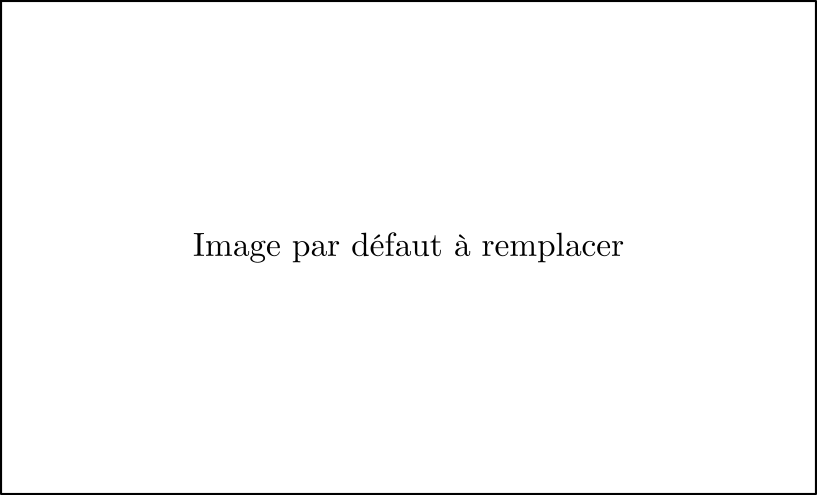
\includegraphics[width=1\linewidth]{default.png}
	\caption{Entrées et sorties du circuit à concevoir}
	\label{fig:entrees_sorties_composant}
\end{figure}

Le tableau ci-dessous récapitule les relations avec leur sens, leur catégorie et leur type.

\begin{table}[H]
	\centering
	\begin{tabular}{|c|c|c|c|c|}
		\hline
		Entités                       & Relation  & Catégorie    & Sens   & Type          \\
		\hline
	\end{tabular}
	\caption{Sens et rôle des signaux}
	\label{tab:entrees_sorties_composant}
\end{table}



\newpage

\subsection{Spécifications fonctionnelles}
Les spécifications fonctionnelles comprennent la liste des fonctions du système
pour l'application (fonctions externes) et la description du comportement du système et
de l'environnement pour ces fonctions \cite{Calvez_2}.

\gap


\subsection{Spécifications opératoires}
\subsection{Spécifications technologiques}